\documentclass[header.tex]{subfiles}
\begin{document}
\title{\plaintitle}

\numberofauthors{3}
\author{%
  \alignauthor{Leave Authors Anonymous\\
    \affaddr{for Submission}\\
    \affaddr{City, Country}\\
    \email{e-mail address}}\\
  \alignauthor{Leave Authors Anonymous\\
    \affaddr{for Submission}\\
    \affaddr{City, Country}\\
    \email{e-mail address}}\\
  \alignauthor{Leave Authors Anonymous\\
    \affaddr{for Submission}\\
    \affaddr{City, Country}\\
    \email{e-mail address}}\\
}




\teaser{
%\begin{figure}
\centering
\includegraphics[width=1\textwidth]{figures/Fig1}
\caption{Sketch\&Stitch walkthrough: (a) A user sketches an art pattern directly on fabric, (b) shes uses \textit{Circuit Stickers} to plan and sketch the circuit, (c) she takes a picture of the design on fabric, (d) the system converts the design into embroidery patterns, and  embroidery machine stitches the patterns using conductive and non-conductive threads, (e) the user attaches electrical components in place of Circuit Stickers.
}
 \vspace{-1em}
\label{fig:Fig1}
}

\maketitle



\begin{abstract}
E-Textiles are fabrics that integrate electronic circuits and components. Makers use them to create interactive clothing, furniture, and toys. However, this requires significant manual labor and skills, and using technology-centric design tools. We introduce \textit{Sketch\&Stitch}, an interactive embroidery system to create e-textiles using a traditional crafting approach: Users draw their art and circuit directly on fabric using colored markers. The system takes a picture of the sketch, converts it into embroidery patterns, and sends them to an embroidery machine. Alternating between sketching and stitching, users build and test their design incrementally. Sketch\&Stitch features \textit{Circuit Stickers} representing circuit boards, components, wire crossings to insulate, and various textile touch sensors such as pushbuttons, sliders, and 2D touchpads. Circuit Stickers serve as placeholders during design. Using computer vision, they are recognized and replaced later in the appropriate embroidery phases. We close with technical considerations and application examples.
\end{abstract}


\category{H.5.2}{User Interfaces}{}

\keywords{\plainkeywords}

\section{Introduction}


Electronic textile technology enables people to create expressive, interactive, and functional textile artifacts for both playful and serious applications.
It combines the visual and haptic expressiveness of textiles with the interactivity and utility of electronic components such as LEDs, GPS receivers, vibration motors, speakers, and touch sensors. At the intersections of technology, art, and fashion, e-textiles have attracted artists, designers, hobbyists, and makers, who are applying this technology in creative and artistic ways \cite{Buechley:2010:LWH:1858171.1858206,CuteCircuit}. 
%https://iq.intel.com/fashion-metamorphosis-meet-the-butterfly-dress/
%http://ezratuba.com/wearable-tech
This has motivated HCI researchers to investigate techniques that enable a wider audience to combine fabrics and electronics into interactive textiles \cite{Buechley2009,5387040}.

In e-textiles, flexible conductive threads, inks, polymers, or  textiles are attached directly to a base fabric, creating \textit{fabric circuits}. They primarily serve to connect electronic components, but can also be used to directly create fabric sensors [], resistors [], antennas [], batteries [], and certain other electronic components. The techniques for building fabric circuits are based on traditional textile methods, such as weaving, knitting, stitching, and printing \cite{castano2014smart}. Creating e-textiles typically involves a) designing or choosing an art pattern, b) planning the layout of components and connections, c) implementing the art pattern and fabric circuit using one of the above methods, d) insulating the fabric circuit where necessary, and e) attaching the electronic components \cite{Buechley2009}.

%Some of these techniques have been successfully adopted by the do-it-yourself community 
% as evident from makers' websites, such as Instructables\footnote{https://www.instructables.com/}, Sparkfun\footnote{https://www.sparkfun.com/} and Adafruit\footnote{https://www.adafruit.com/}. But these techniques have some constraints.
%More websites: https://www.lib.ncsu.edu/softcircuits



Current e-textile fabrication techniques are predominantly manual \cite{Kazemitabaar:2017:MTA:3025453.3025887}. As a result, executing a design becomes labor-intensive and requires high skill levels as the number and density of electrical connections and components increases. Debugging a fabric circuit is only possible after the user has invested considerable time in fabrication. In addition, current techniques demand a separate step, tools, and materials for insulating the electrical connections, which is necessary to achieve a functional artifact without accidental shortcuts during use.
Observing participants in our e-textile workshops, we found that this laborious multi-step process often forces people to make a trade-off between the visual and functional aspects of their design, and impedes improvisational fabrication. %people during early design explorations. 
%enable users to focus and invest their time on the visual and functional aspects of their project.


% We analysed more than 70 e-textile projects on the mentioned websites and found that makers make a trade-off between the fidelity of the artistic pattern and the functionality of the artefact. 


In this paper, we present \emph{Sketch\&Stitch,} an interactive embroidery system that enables users to create e-textiles by sketching on fabric (Fig.~\ref{fig:Fig1}). It uses a computerized embroidery machine as a digital fabrication tool to handle the two most laborious steps when creating e-textiles, stitching and insulation. Sketch\&Stitch features \textit{Circuit Stickers}, printed adhesives representing elements users can embed into their design, from circuit boards and components, to wire crossings to insulate, to various textile touch sensors. These stickers guide the user while drawing circuit traces to ensure reliable electrical connections, and are recognized using computer vision, automatically generating stitching patterns for sensors and insulations, for example.

In Sketch\&Stitch, a user begins by sketching an art pattern on the workpiece fabric using colored fabric markers. She plans the placement of components using Circuit Stickers and draws connections. When the user is ready to execute the design, the system takes a picture of the sketch, converts it into embroidery patterns, and sends them to the embroidery machine. 
%The embroidery machine's embedded display allows the user to verify the patterns and make minor adjustments before stitching is started. 
The user may repeat these steps to review and test parts of their art and circuitry incrementally. After embroidery is complete, the user replaces Circuit Stickers permanently with their component counterparts, using one of three attachment techniques we describe.

In summary, this paper makes the following contributions:
\begin{itemize}
    \item Sketch\&Stitch, a new approach and system prototype to create e-textiles by drawing directly on the fabric,
    \item Interaction techniques and embroidery patterns that let users include circuit boards, components, insulation, wire crossings, and a variety of fabric sensors using Circuit Stickers,
    \item Technical recommendations for materials and stitching processes to create e-textiles using computerized embroidery machines.
\end{itemize}

In the remainder of this paper, we first briefly introduce the reader to the particular features of computerized embroidery machines that are relevant for this work. After reviewing related work, we present Sketch\&Stitch and its interaction design. We illustrate the extensions we added to Sketch\&Stitch beyond the basic system that enable a wider range of practical applications, and walk the reader through a concrete example. After providing details on the software implementation and recommendations for materials and stitching techniques, we present several example artifacts created using our system, and close by discussing the current limitations of Sketch\&Stitch and opportunities for future research.

% Machine embroidery has bloomed entering homes, makerspaces and design studios of crafters, hobbyists and DIY.

% \url{http://www.strategyr.com/MarketResearch/Sewing_Machines_Market_Trends.asp}

% \url{http://robyns.world/2015/06/13/infographic-sewing-machine-day/}


\subfile{RelatedWork}


\section{Embroidery Machine In Personal Fabrication}
Computerized embroidery machines became available for homes and small business in the 1980s. At prices between 500 and 15,000 US Dollars, they have become a tool frequently found in schools, fab labs, maker spaces, and small businesses \cite{lipson2010factory}. 
%An embroidery machine retails at 500 - 15,000 USD.
Embroidery machines use a hooping system to hold the framed area of fabric taut under the needle and move it automatically on an X and Y axis to stitch embroidery patterns. A presser foot, a metallic attachment that surrounds the needle, holds the fabric flat during embroidery to prevent it from rising and falling with the needle. A control panel and embedded display enable users to start-stop the machine, control thread tension, change stitching speed, view embroidery patterns and make minor adjustments (e.g., re-positioning, scaling, rotating, sequencing). Commercial embroidery machines can stitch up to 1000 stitch/min.


 \begin{figure}
\centering
  \includegraphics[width=0.8\columnwidth]{figures/EmbroideryWorkflow}
  \caption{Image digitization in embroidery software: (a) export image, (b) separate into color layers and assign thread color, (c) generate tool path, (d) final embroidery pattern }~\label{fig:EmbroideryWorkflow}
  \vspace{-2.5em}
\end{figure}

Embroidery machines come with proprietary software that runs on the user's computer. Embroidery software digitize images into digital embroidery patterns and generate a tool path for the machine. The path dictates how an embroidery hoop moves under the needle. It includes stitch patterns, thread color changes, and jump stitches when traveling between different stitch objects. To optimize tool path generation, embroidery software separate design objects into multiple layers based on color (Figure \ref{fig:EmbroideryWorkflow}). This reduces the number of times a commercial embroidery machine has to stop and prompt the user to manually change thread color. Jump stitches also require manual trimming at the end on an embroidery. To reduce these jumps, embroidery designers re-program embroidery patterns, manually sequencing stitch objects and individual stitches. 
%Industrial embroidery machines can change thread colors automatically. A large number of jump stitches in a path is a sign of bad design digitizing. Expert embroidery designers re-program embroidery patterns, manually manipulating the sequence of individual stitches to influence the tool path and reduce jumps. 
An embroidery machine reads a digitized embroidery pattern from a memory card or a computer connection, recognizes color layers and stitches them sequentially.

%Virtual hoops help the user position, orient and scale a design relative to physical hoops. 
%Some software tools allow the user to print a design inside a virtual hoop in life-scale to assist the user in aligning the physical hoop on the workpiece fabric.

Similar to advanced CAD tools, embroidery software require a relatively steep learning curve. They offer a large number visual design options as well as specialized tools for manipulating stitch patterns, such as a parametric stitch designer. % and pull compensation options. 
In addition, the user-interface language of these tools is targeted at users who posses a level of knowledge in threads, fabrics, and embroidery.
%and the basic dynamics of the embroidery machine.





\section{Sketch\&Stitch}
Sketch\&Stitch utilizes an embroidery machine to take over the laborious tasks in e-textile fabrication---stitching and insulating conductive traces. Yet, it maintains the physical and direct interaction between the user and the workpiece fabric during the creative tasks---designing and planning visual and functional patterns. 
%By this, the system aims to ... 
%reduce the entry barrier to e-textile fabrication and 
%encourage creative and improvisational and creative designs.

Sketch\&Stitch setup comprises a commercial embroidery machine, a smartphone attached to a camera mount, and two bluetooth buttons for user interaction. The system includes a smartphone app for color calibration and image capture, and computer software for image processing, and for communicating with embroidery software and machine.

Sketch\&Stitch design pipeline was developed with designers and makers in mind. %and artists
It enables them to convert a idea sketched on fabric into an interactive embroidery without having to interact with computer screens or CAD tools. Unlike circuit layout tools (e.g., Eagle or Fritzning), Sketch\&Stitch enables users to draw electrical connections in free artistic forms adding design interest to circuitry. Physical sketching provides users with continuous representation of their workpiece and helps them establish a closer relation with the materials (fabrics, threads, electronics) to better understand their properties and nuances \cite{}. Users interact with Sketch\&Stitch using colored markers and \textit{Circuit Stickers}. It is thus designed for improvisational and iterative prototyping during early design stages. 

 
%Potentially, it can lowers the barrier for designing e-textiles
%feedback on how a design (i.e., position, orientation, scale) will appear

%asses the visual design, test circuit layouts, or evaluate how the fabric material will behave when electrical components are attached to it
%It automizes the digitization of designs into embroidery patterns, and includes new patterns for conductive thread. 


Circuit Stickers are symbolic images printed on adhesive sheets of paper. %They have the same shape, size and name of circuit elements they represent.
They represent circuit elements that can be embedded into fabric during and after embroidery. Circuit Stickers were developed to (a) overcome the limitation of the low hovering presser foot in commercial embroidery machines and the risk of breaking the needle or hardware if they come in contact, and (b) to signify custom multi-layer embroidery patterns that cannot be skecthed in 2D.

Sketch\&Stitch supports two types of stickers: Component Stickers, which serve as placeholders for hardware electronics, such as circuit boards, LEDs, motors, speakers; and Embroidery Stickers representing custom embroidery patterns for touch sensors and shielding. Circuit Stickers are designed to help users plan and sketch a circuit with ease and precision. The adhesive backing invites for exploring different placement layouts, and holds the stickers in place during sketching and stitching. After capturing their design, users remove Embroidery Stickers for the machine to embroider in place. After embroidery in complete, users remove Component Stickers and replace them their hardware counterparts, using one of three attachment techniques we describe.
%Some stickers include grooves to guide users' traces to ensure reliable electrical connection with the added units. 


The general end-to-end workflow of Sketch\&Stitch allows users to a) sketch an art pattern directly on fabric with a textile marker, b) plan and place Circuit Stickers and draw connections between them, c) capture fabric design with a camera, d) stitch the design on an embroidery machine, and finally e) attach electronics onto fabric.

%  We aim to make e-textile creation accessible for emerging designers, hobbyists, crafters, and makers.
%To keep the traditional craft ways of entirely working on the physical workpiece, we developed a pipeline that enables users to sketch the design and plan the circuit directly on fabric. This pipeline 
% Simulating the traditional craft ways of directly interacting with the physical form using tools opens up a range of new creative possibilities [].
%Disconnect between physical and digital: There are numerous sources of variability in textile materials that can make a digital representation unstable, regardless of how good the simulation is.
% More agency and control over the final outcome [Being the Machine: Reconfiguring Agency and Control in Hybrid Fabrication].




\subsection{Sketching the design}
Drawing on fabric is an established form of art. It is also used to design patterns for manual embroidery. 
%Freehand sketching is the way users convey their design ideas to the system, and color, is the interaction language. 
Sketching on fabric utilizes a simple and masterful tool, a marker or a pen, that enable users to express themselves freely without the constraints of design applications \cite{schweikardt2000digital}. 


To start sketching on fabric, a user secures it in an embroidery hoop of desired size. The hoop holds the fabric flat and taut, and frames the design location on the workpiece. Next, she selects her marker color palette and follows color calibration instructions on Sketch\&Stitch mobile app. The system preserves three distinct colors---\textit{trace color} and two \textit{sticker colors}---and one optional \textit{insulation color}. The remaining colors, \textit{art colors}, can be used to draw the art pattern. For the purpose of versioning, the user should avoid using thread colors from her marker palette. Sketch\&Stitch uses colors instead of annotations for user-system communication to avoid imposing design constraints on freehand sketching and keep the design uncluttered. In addition, Sketch\&Stitch uses colors to enforce the sequence of pattern execution when communicating with embroidery software. For example, the system sequences all objects in trace color marker to be stitched first using conductive thread, followed by objects in art colors using non-conductive threads.


%The user can draw any lines and shapes. 
The user can start with either pattern---art or circuit---and alternate between them. When drawing circuit traces, the user should keep using the trace color marker from the calibration process. If the users wants to \textit{undo} any markings, washable fabric markers allow her to erase color by simply patting on fabric with a damp piece of cloth. The amount of details the system can recognize in a design depends mainly on the quality of image capture (camera and lighting) as well as fabric texture and maker quality (tip and color consistency). %When drawing circuit traces, the user should maintain the 2.5 mm spacing between adjacent traces. 
%The quality of embroidery depends highly on the quality of the captured image. Factors that affect the quality of an image include camera resolution, light setup and shadows, the flatness and texture of fabric, the quality of markers, and the amount of presser applied to makers while sketching.

A design does not need to be complete before it can be stitched. At any point, the user can take a picture of the fabric, secure the hoop in an embroidery machine, and start the stitching process. This enables users to evaluate and test their design early on.  Sketch\&Stitch supports \textit{incremental design}. If a user wants to sketch on an embroidered fabric, she first captures a picture of the current design, and then proceeds sketching.


\subsection{Adding Electronics}
Sketch\&Stitch users use Component Stickers on fabric to serve as placeholders for the hardware electronics they want to embed in their design. As we mentioned before, embroidering while hardware components are on fabric is very challenging for most embroidery machines due to the low hovering height of the presser foot (\~ 1 mm). For context, LilyPad PCBs are 0.8 mm thick, and with attached SMD components the total thickness is more than 2 mm. Moreover, embroidering near hardware requires precise alignment between virtual and physical sketches to avoid the needle from punching into the hardware. 

Figure \ref{fig:BlackStickers} shows example stickers for the LilyPad kit. Stickers have the same shape, size, and name of their physical counterparts. LilyPad components have exposed conductive plates on the top and bottom of the PCB. The grooves near the pin holes guide the user to ensure that circuit traces extend under the component and create sufficient contact surface for hardware attachment. Users can access these stickers from Sketch\&Stitch mobile app and print them on adhesive sheets of paper using any printer. The sticker are tinted with sticker colors (in this example, black and white). Every time the user wants to use a sticker, she can cut it into shape, peel its backing, and adhere it to fabric. Using the trace color marker, she can draw circuit traces from and to the stickers. 
%The user may use a vinyl cutter to quickly cut them into shape. 
Circuit Stickers can be created for any off-the-shelf electronics. The only constraint is that they must have a pitch of 2.5 mm or wider between their leads (we discuss this in X). 


\begin{figure} [h!]
\centering
  \includegraphics[width=0.5\columnwidth]{figures/BlackStickers}
  \caption{}~\label{fig:BlackStickers}
  \vspace{-2.5em}
\end{figure}

\subsection{Attaching Electronics}
%We mainly considered sewable components, and components with flat pads on the wrong side of the unit.




After embroidery is complete, the user replaces Component Stickers with hardware electronics. 
%Sketch\&Stitch simplifies this step by stitching the contact surface  d. 
%Attaching hardware circuit boards and components to fabric is one of the main challenges in e-textiles. Researches have explored several techniques including soldering [], special soldering [], manual sewing [], breads [], ...
We describe three techniques for attaching sewable electronics to fabric: First technique uses M3's Z-tape, a double sided adhesive that conducts in the Z-dimension when pressed down. A piece of Z-tape is applied to the back of a component, the component is then aligned and adhered over the stitched contact surface on fabric. By pressing the component on fabric, connections between pins and stitches are created. This technique is suitable for testing and prototyping a circuit, and for fabrics with low movement requirements. 

%We do not know if Z-tape can hold components with legs, we only tested with flat pads.

\begin{figure}
\centering
  \includegraphics[width=0.7\columnwidth]{figures/LilyStitch}
  \caption{}~\label{fig:LilyStitch}
  \vspace{-2.5em}
\end{figure}

The second technique utilizes an embroidery machine. We developed the \textit{Lily Stitch} for attaching components that have 3 mm diameter pin hols via embroidery. The stitch is an M shape (9 mm length, 0.8-1.2 mm width) stitched with a single running stitch (9 mm length), and tie-in and -off knots on the wider end. The M shape was selected, as opposed to a line shape, to avoid punching the needle several times in the same position on fabric, which can enlarge the hole and make the connection weaker. 
%Tie knots need space that 3mm is not encough for them
The length of the lily stitch accounts for (a) the distance between the center of a pin hole and outer edge of the PCB (\~ 4 mm), and (b) the distance between needle point and presser foot outer edge (\~ 5 mm). Reducing the stitch distance leads the presser foot to push against the edge of the PCB when stitching close to it. And increasing the distance weakens the strength of the stitch.

Figure \ref{fig:LilyStitch} shows a custom embroidery pattern for embroidering LilyPad Arduino USB - ATmega32U4 Board. Lily stitches were sequenced manually to prevent the presser foot from traveling over the component during embroidery. This technique is very reliable and efficient for attaching sewable electronics. However, it requires a millimeter accurate alignment between the physical component on fabric and the embroidery pattern. If an embroidery machine does not support such accuracy, one can start by stitching part of this pattern on fabric, align the component on fabric based on the stitches, and restart the pattern embroidery. Sketch\&Stitch stores embroidery patterns for stitching LilyPad components on the embroidery machine. The user can access them from embroidery machine's display.
%We recommend embroidering the hardware after the art and circuit patterns have been fully embroidered to avoid travel stitches.

The last technique is using the \textit{button sewing} presser foot in sewing machines. In this technique the user has to manually align each hole on the PCB under the foot. This requires skill but can become efficient. The user can also use the status-quo method of manually sewing into the holes using conductive thread. 
%And part stickers
The results of a sewing machine and manual sewing can be as reliable as the embroidery machine's but the former techniques require more manual labor and time.


\subsection{Insulating circuit traces}
Insulating circuit traces, especially in wearable e-textiles, is paramount for their functionality. Textiles are flexible materials. Exposed traces may come in contact with each other as fabric folds or bends creating shorts or undesired signals. Buechley et al. \cite{Buechley2009} proposed couching---stitching on thread over another---as an organic insulation technique for fabric circuit traces. However, they noted that sewing machines may leave gaps in the top stitch making it an unreliable cover for the underlying conductive thread. Computer-controlled embroidery machines are particularly more qualified than sewing machines at maintaining a consistent couching stitch. 


In Sketch\&Stitch the user can selectively mark circuit traces that she wants to insulate by drawing them using the insulation color marker. The system duplicates all objects colored in the insulation color and stores them in two design layers. The layers are color tinted to be mapped to specific stitch types on embroidery software. We describe the color tinting process in Implementation section. While couching circuit traces has functional advantages, it can have two pitfalls: (a) it can add a pronounced visual impact to the design since, and (b) the build-up of stitches can reduce the flexibility of the base fabric especially if applied to several traces in a small area.



%anto be stitched sequentially---the bottom layer using conductive thread, and the upper layer using non-conductive thread. 
%Sketch\&Stitch user a zigzag stitch (1.5 mm width, 0.3 spacing) to anatomically insulate circuit traces. 




\subsection{Handling Crossing Traces}
\begin{figure}
\centering
  \includegraphics[width=0.7\columnwidth]{figures/BridgeStitch}
  \caption{}~\label{fig:BridgeStitch}
  \vspace{-2.5em}
\end{figure}
As the number of circuit elements increases in a design, circuit traces crossing each other becomes inevitable. Dunne et al. \ref{} suggested manipulated the tension of thread to allow two conductive threads to crisscross without coming in contact with each other. However, this technique does not provide a fail-safe insulation, especially when pressure is applied to the intersection point. In addition, by adjusting the thread tension to be too high or too low, the strength and appearance of the stitches will be impaired. This technique may also lead to ``thread birdnesting'', which causes the thread to tangle and the machine to stop.  
%various fabric-thread combinations require different tension settings and changing these settings may affect the appearance and strength of the stitches. 
Sketch\&Stitch provides users with an Embroidery Sticker, the \textit{shield sticker}, to signify crisscrossing traces on fabric. The user places the sticker over the intersection point and aligns the traces to the dotted lines (Figure X). Self crisscrosses of conductive thread are safe and do not need to be handled.
%This ensures that the bridge patterns with overlap with the traces. 


The fiducial marker in the \textit{shield sticker} is used to localize it and replace it with three design layers: bottom layer contains a line segment for connecting one trace, middle layer contains a line segment for insulating that trace, and top layer contains an M shape object to connect the perpendicular trace. The layers are color tinted to be mapped to specific stitch types on embroidery software. The top layer is mapped to a custom stitch, \textit{Bridge Stitch}, the is similar to the Lily Stitch expect for two minor differences: (a) the width of the stitch is consistent (0.8 mm), and (b) the tie-in and -off knots are each on one end of the stitch. The Bridge Stitch is used to connect two separate segments (< 9 mm apart) without stitching between them. 


%The layers are tinted in a color scheme that maps to specific stitches---triple running, zigzag 0.3/2.0, and a \textrit{bridge stitch}, respectively. And converted in embroidery software to a bridge embroidery pattern (Figure \ref{fig:BridgeStitch}).
%The bridge stitch, the top layer in the bridge pattern, is a single running stitch (9 mm long) stitched in an M shape. 

%3.7 mm





\subsection{Adding Interactivity}
% \begin{figure}
% \centering
%   \includegraphics[width=0.6\columnwidth]{figures/RedStickers}
%   \caption{}~\label{fig:RedStickers}
%   \vspace{-2.5em}
% \end{figure}
Besides hardware electronics, users can use an Embroidery Sticker, \textit{sensor sticker}, to embroider touch sensors directly on fabric. Below we describe three touch sensors an embroidery machine can create using conductive thread: a pushbutton, a 1D slider, and a 2D touchpad (Figure \ref{}) .
%actuators, e.g., by couching a shape memory alloy wire, and various touch sensors, as we will demonstrate in this section.

The pushbutton, is the simplest sensor---by connecting a segment of conductive thread to a capacitive sensing circuit, a pushbutton is created. The circuit can sense when the user's finger or body is in contact with the thread (touch) or not (no touch). Users can design pushbuttons to have a larger surface and an artistic shape by drawing and filling a shape with a trace color marker. A resistive pushbutton can be created using two conductive traces 3-4 mm apart, one trace grounded. Using this simple technique, users can create physical widgets of custom shapes or make their art pattern touch-enabled by drawing conductive traces as part of the design itself.

%When the user touches the two segments at the same time, a resistive sensing circuit registers a touch.

A 1D slider can be implemented by placing pushbuttons next to each other. A resistive circuit enables a slider with coarse resolution. A capacitive circuit can enable a higher resolution by interpolating the position of a finger based on the amount of surface area it covers and its influence on the capacitance of neighbouring buttons.

% to determine more than one capacitive threshold for a single button. As the user's body comes in contact with more surface o with a capacitive sensor is interacted with by the user, the larger the capacitance will be. 

A matrix of buttons, where each button is connected to one pin in a controller, can be used as a 2D touchpad. 
%offers the ability to detect all buttons being pressed at the same time, i.e., multi-touch. 
However, a 4$\times$4 touchpad will require 16 pins and traces. This can complicate the wiring and require additional hardware. Instead, using a grid layout provides a sensor surface area that is capable of detecting individual buttons, simple gestures, and sub-sensor point detection. A grid sensor requires fewer pins (8 in case of 4$\times$4 pad) and lower power than the individual button scanning. 
%However, it cannot support multi-touch. A grid layout can be connected to a capaciiuve or resistive circuit. But due to the low resistivity of the human finger, not all hardware can detect a direct touch. One alternative is to use pinching as an input technique. Hamdan et al. [] were able to detect the location and angle of a pinch on a matrix of resistive textile buttons using simple machine learning algorithms.

Based on design recommendations from Texas Instruments \cite{}, we designed an embroidery pattern for a touchpad sensor (Figure X). The \textit{sensor sticker} has fiducial markers at the intersections points of the grid. The system replaces these with the same three layer design of a \textit{shield sticker}. The sensor grid is tinted with the trace color and treated similar to hand sketched circuit traces.

Sketch\&Stitch user can print the \textit{sensor sticker} on a sheet of adhesive paper, cut it into a convex shape to create a slider or a touchpad, peel and stick it on fabric, and use a trace color marker to draw connecting traces from the sensor grid to a the pins of a controller. After capturing fabric design, the user removes the \textit{sensor sticker} for the embroidery to stitch the pattern in place.

%The grid was designed based on the recommendation of Texas Instruments 


% constructed by “opening up” a capacitor structure so that the
% electric field can be interfered with by a conductive foreign object, in this case, a fingerWhen a conductor, e.g., a finger,
% comes into the area above the open capacitor, the electric field is interfered with causing the
% resulting capacitance to change. The coupling of the conductive finger into the capacitive sensor
% increases the capacitance of the structure beyond the baseline capacitance, the capacitance of
% the sensor with no touch. By continuously measuring the capacitance of the sensor(s) in the
% system and comparing each result to a predetermined baseline capacitance, the system
% microcontroller can determine not only on/off button functions for each sensor element but also
% “amount” of press used for more complex interfaces such as positional sliders. 
% The base capacitance of such a design is affected by stray capacitances on the PCB as well as
% potentially other environmental effects such as temperature and humidity. Therefore, the
% detection system needs to constantly monitor and track this variation for correct comparison to
% touch events. 



 

\subsection{Concealing Traces and Components}
Our system offers four techniques to conceal circuit traces and hardware components in a design: the first is drawing circuit traces to be part of the art pattern. The second is drawing circuit traces close to art outlines. 
%The spacing constraint of 2.5 mm need not to be applied between conductive and non-conductive threads. 
While this technique does not hide the traces, it makes them less visible and obvious. 
%since the width of art stitches is relatively larger than trace stitches.

The third technique is camouflaging traces by insulating them with a thread color that matches the color of fabric \ref{}. Traces will not be hidden completely, but depending on the desired application, this technique may be sufficient to occlude electrical connections. 

The forth technique allows users to hide fabric circuits and hardware components completely. This technique uses two layers of fabric: top layer one for sketching art patterns, and the bottom layer for sketching circuit traces, and adding and attaching Circuit Stickers. The two fabrics are captured and embroidered individually. At the end of embroidery, the user attaches hardware electronics to the bottom fabric and manually layers the fabric on top of each other. For, components that need to be visible on the surface, e.g., light sensors and LEDs, the user may cut the top fabric at their location. Another option is attach these parts on the top fabric and use one of the suggested thread-based attachment techniques to connect them to their contact surface on the second layer. This technique can also be used to create multi-layer textile circuits \ref{}, with an additional if an insulator, e.g., non-conductive fabric, between any two conductive layers. 







\section{Walkthrough: Wearable Mandala}

\begin{figure}
\centering
  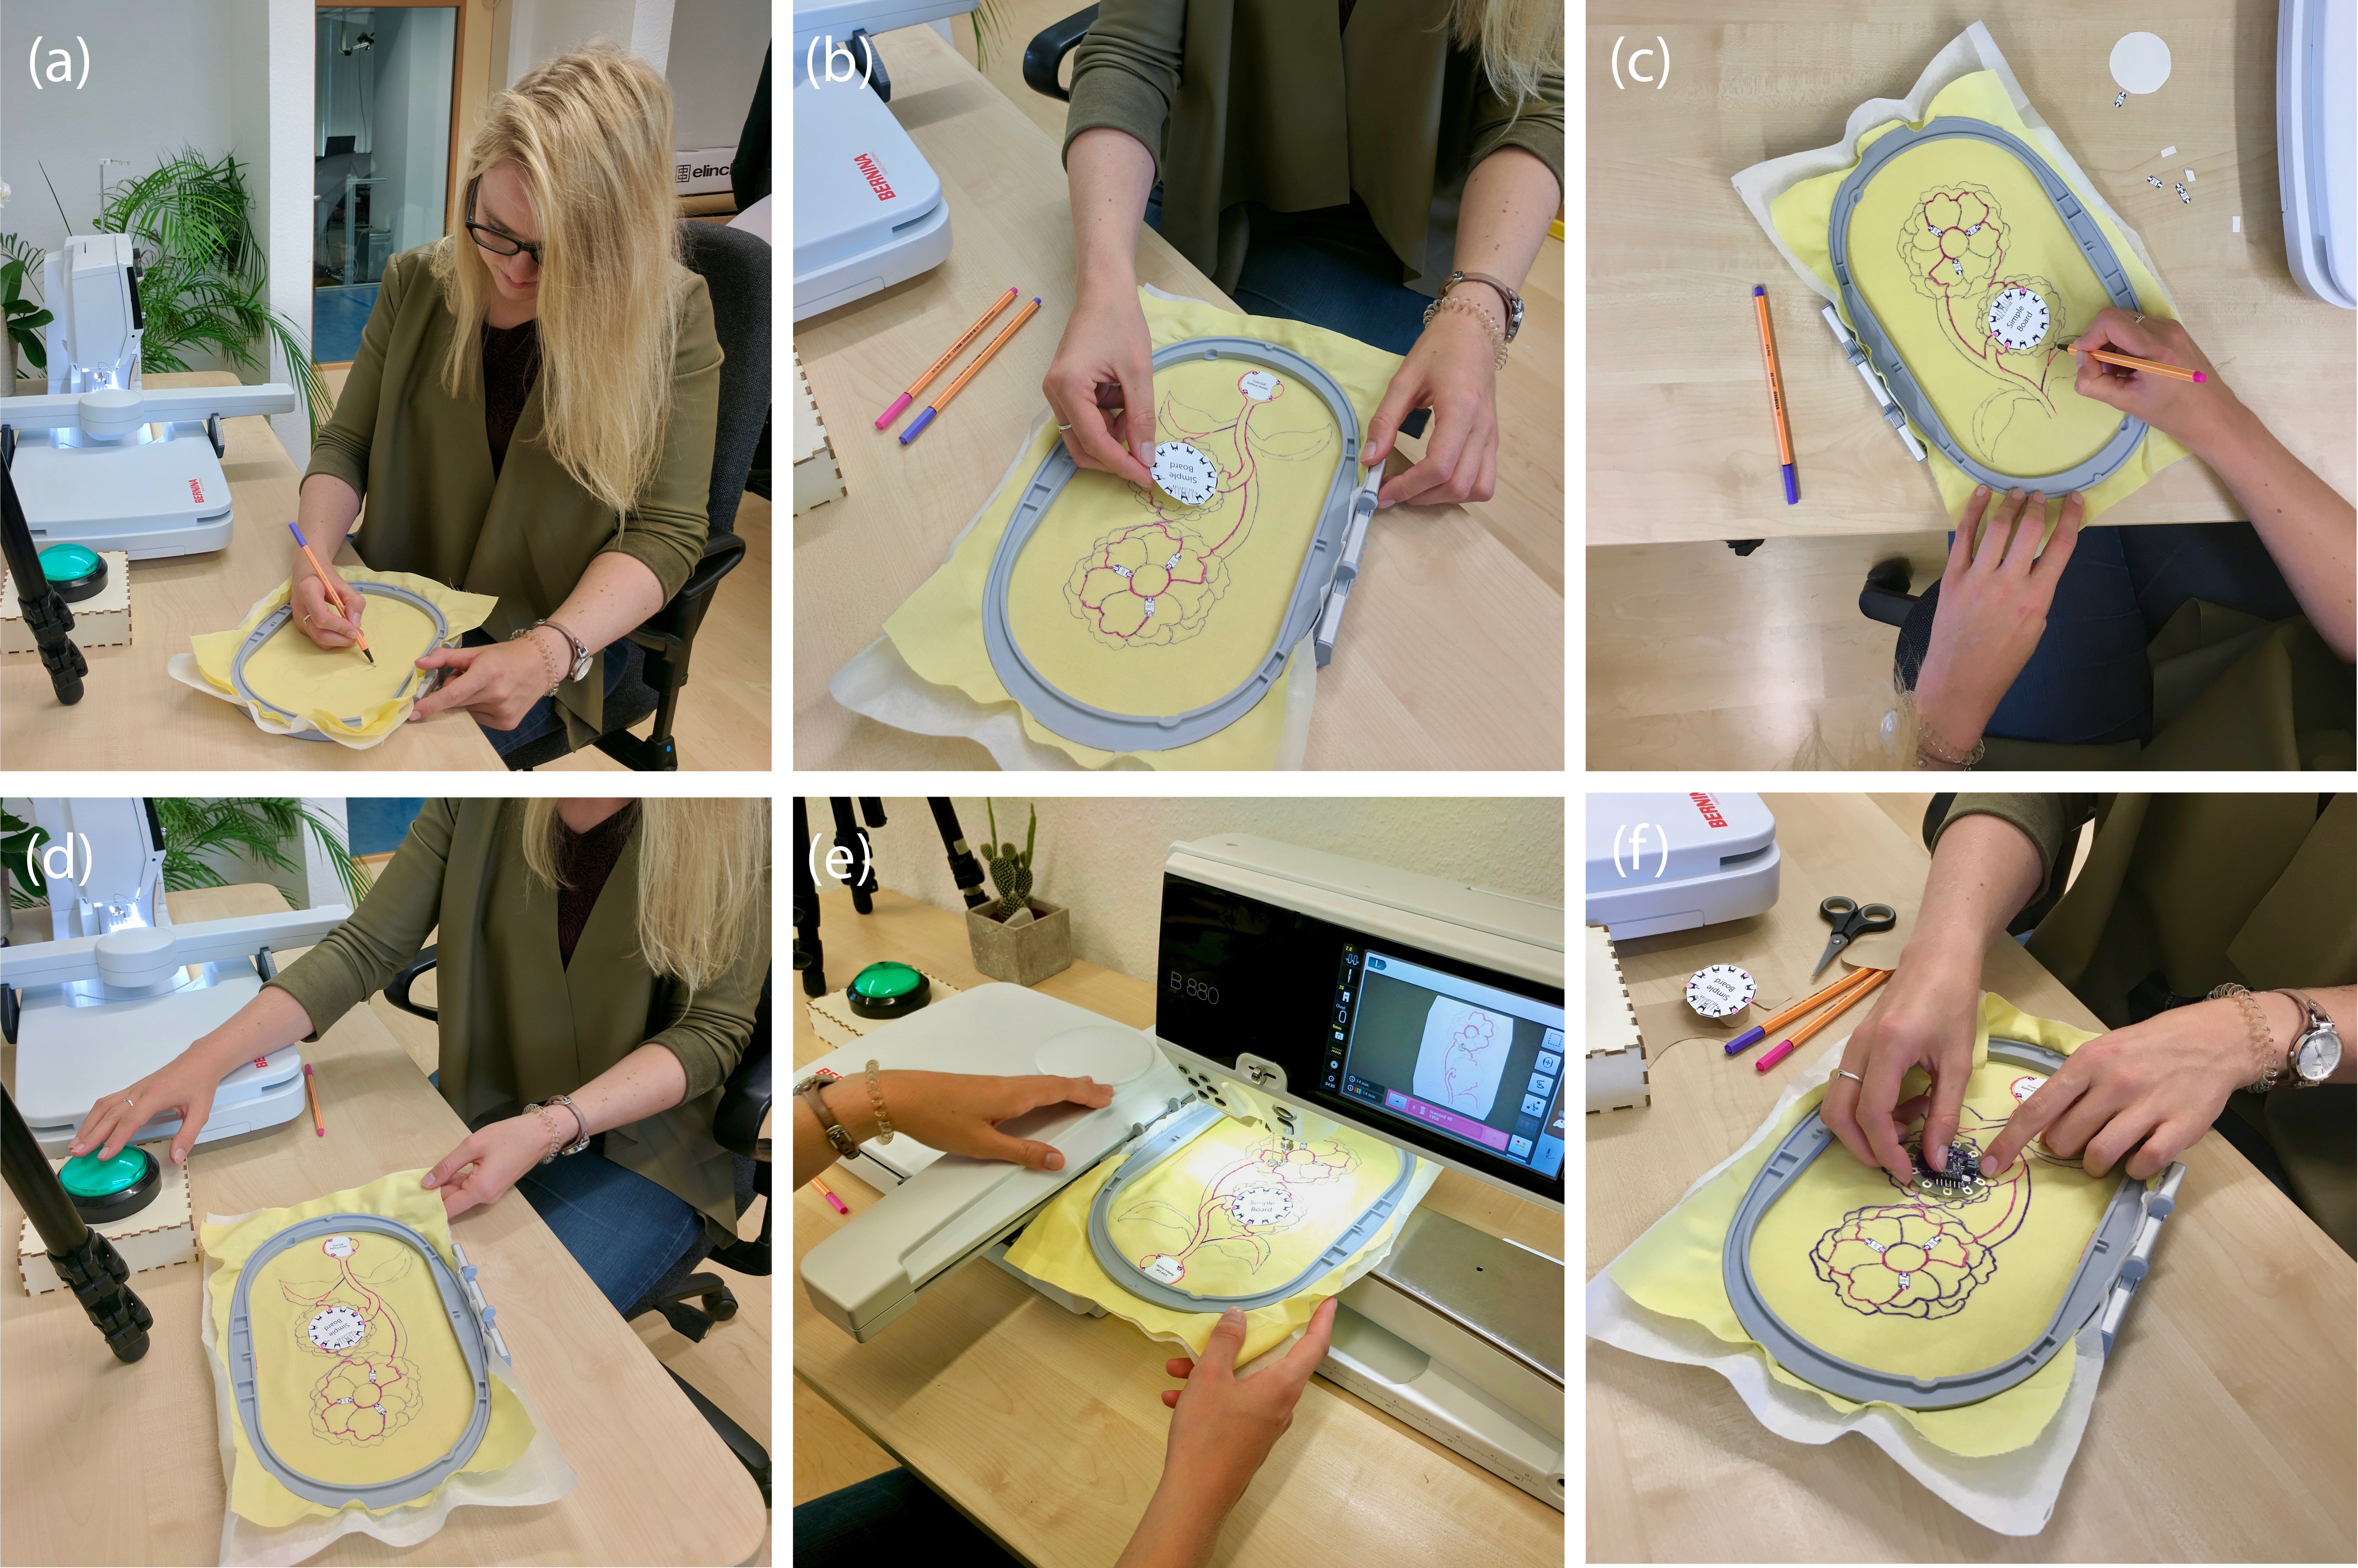
\includegraphics[width=0.9\columnwidth]{figures/Walkthrough}
  \caption{}~\label{fig:Walkthrough}
  \vspace{-2.5em}
\end{figure}
In the following, we illustrate Sketch\&Stitch's basic design pipeline at the example of a wearable mandala. The mandala includes 2  Pixel boards, 8 LEDs, 1 battery holder, and 1 LilyTiny
%ATmega32U4 Board 
from LilyPad kit. Figure X shows the final outcome and the intermediate steps required to produce it.


\subsubsection{Sketching and placing Circuit Stickers}
At the beginning, the user hoops her fabric and calibrates her marker color palette using Sketch\&Stitch mobile app. 
%She places her fabric and markers under the camera mount, and presses  
%prints Circuit Stickers on adhesive paper using her home printer. She cuts the stickers she need for the project---board and pixels. Then, she frames the center of a T-shirt in an embroidery hoop. 
Using one of the art color markers, the user starts by drawing the outline of a mandala. She places Circuit Stickers inside the mandala to estimate their size and location. Once satisfied with the arrangement, she peels the stickers' backing and adheres them to fabric. Using the trace color marker, she draws circuit traces between the component stickers. When the user makes a mistake sketching, she can simply pad a damp piece of cloth on fabric to erase the markings. 

\subsubsection{Capturing and embroidering design}
When the user is ready to embroider her design. She presser on a button next to the camera mount and the system captures a picture of the design inside the hoop. The user then secures the hoop in the embroidery  machine and uses the embedded display to view the digital embroidery patterns of her design---art and circuit patterns. She threads the embroidery needle with conductive thread and starts the embroidery. The machine begins embroidering the circuit pattern. Once it is done, it prompts the user to change threads. The user threads a non-conductive colored thread and starts the machine again. 

% \subsubsection{Debugging}
% After embroidery, the user removes the hoop from the machine, and trims jump stitches. She places the board and pixels over the fabric to verify the alignment of their pins and contact surface. She uses a digital multi-meter to test her traces for any shorts or undesired connections. 

% \subsubsection{Designing Incrementally}
% She cuts a sensor sticker (3$\times$4), and adheres it on fabric. She draws traces from the sensor to the board. Switching to the purple marker, she completes the design of the mandala. She take a picture of the new design, removes the sensor sticker, secures the hoop in the machine, and starts the embroidery machine stitching the sensor and remainder art pattern. 

\subsubsection{Attaching electronics}
After the embroidery is complete, she removes the hoop from the machine, and trims jump stitches using a scissor. She cuts and peels a piece of Z-tape and applies it on the back of the hardware components. Guided by Circuit Stickers, she determines the location and orientation of each component. She removes the stickers and adheres the components on fabric over their contact surface. Finally, the user inserts a battery in the battery holder and sees her design augmented with light.

%become Finally, the user uses, e.g., Arduino IDE, to program the functionality of her e-textile.



%The user is free to perform this step in any environment since her input is not tracked in real-time. 

\subfile{Implementation}


\section{Embroidering with conductive thread}

In this paper we use Bernina 880B\footnote{https://www.bernina.com/880} embroidery machine and software (DesignerPlus version 8) with Shieledx 117/17 dtex 2 ply silver sewing thread (linear resistance < 30 $\Omega$/cm). 
%http://www.shieldextrading.net/products/yarns-threads/
This thread can carry current for power and signals. The embroidery machine requires two types of thread: a top thread (or fashion thread) which appears on the surface of fabric, and a bobbin thread which runs on the wrong side of the fabric to pull the top thread down. We investigate using conductive thread as a top thread. While working with the conductive thread we adjusted the embroidery machine as follows: we set the stitching speed to 300-400 stitch/min to reduce the heat and friction that is associated with high speeds. We reduced top thread tension by 0.25 degrees from fabric recommendation, and used a light weight bobbin thread (60wt).


We performed a battery of experiments to identify stitching parameters for conductive thread. 

\paragraph{Resisitivity}
First, we tested the effect of stitch type on the resistivity of circuit traces. Unlike traditional copper wires, the resistivity of conductive threads is relatively high and plays a key factor in the layout of fabric circuits. The length of an electrical connection influences the amount of current that can be delivered to the components---longer connection draw more current and require more power. One way to reduce the resistivity of conductive threads is to increase the number of connections between the conductive fibers that compose the thread. In Figure x we show how stitch types can be used to adjust resistivity. Dense or wide stitches, such as satin or zigzag, reduce the resistivity of a line compared to loose or narrow stitches, such as single and triple running. But wide stitches consume more thread and have a more pronounced appearance on fabric compared to narrow ones. For the purpose of our system, we chose triple running stitch as the default for embroidering circuit traces and sensors.


\paragraph{Spacing}
 \begin{figure}
\centering
  \includegraphics[width=0.8\columnwidth]{figures/Spacing}
  \caption{}~\label{fig:Spacing}
  \vspace{-2.5em}
\end{figure}

Next, we tested the minimum possible spacing between adjunct traces. The goal was to find the minimum distance that can be between any two exposed conductive traces, even after handling the fabric. Figure~\ref{fig:Spacing} depicts our experiment. We tested the connectivity between the traces instantly after embroidery and again after handling the fabric for several days. We found 2.5 mm spacing to be a safe minimal distance. The figure shows fraying fibers connecting lines at 1.0 and 1.5 mm. Tie-in and -off knots secure the ends of embroidery threads. They are wider than a triple running stitch, and when the thread is cut at these points, it frays. On the wrong side of the fabric these knots connected traces at 2 mm spacing.



\paragraph{Insulation}
\begin{figure}
\centering
  \includegraphics[width=0.7\columnwidth]{figures/Insulation}
  \caption{}~\label{fig:Insulation}
  \vspace{-2.5em}
\end{figure}
Finally, we evaluated insulation stitches that can cover and prevent circuit traces for creating electrical connections even if they are in physical contact. 

The zigzag stitch (a back-and-forth stitch) is the most common for couching---stitching one thread over another. It is defined by two main parameters: width of the stitch and spacing between threads (density). We manipulated these parameters to find the stitch that best insulates a triple running stitch of conductive thread. 
%Insulating conductive thread is challenging due to its fraying properties. 
Our goal was to find a trade-off between the reliability of insulation, and the width and destiny of the stitch. A wide insulation would dictate the smallest distance between adjunct traces and might have a pounced visual effect on the design. A highly dense insulation requires more thread and could reduce the flexibility of the underlying fabric, especially if applied to several traces in a small area.

Figure \ref{fig:Insulation} illustrates the tested parameters and summarizes the results.
We evaluated the insulations as follows: we overlaid the insulated traces over non-insulated conducive traces, and applied different amounts of pressure (2, 6, 10, 14, 18 N) at 5 equidistant points along each trace. An insulation stitch of 1.5 mm width and 0.3 mm spacing satisfies our technical and design requirements. It also insulates conductive traces on the wrong side of the fabric. Based on this result, two insulated traces can be spaced closes, at 2 mm.




\section{Example E-Textiles}

\subsection{On-Hour Nap Pillow}
\begin{figure}
\centering
  \includegraphics[width=0.7\columnwidth]{figures/Insulation}
  \caption{}~\label{fig:Insulation}
  \vspace{-2.5em}
\end{figure}
The one-hour nap pillow is composed of a touch sensor that detects when a person first sleeps on the pillow and after one hour of continuous contact awakens him gradually using different vibration patterns. The user can snooze the pillow by shaking it. An accelerometer signals a 5 or 10 minutes snooze based on shaking intensity. The pillow is constructed using two layers of fabric: the lower layer contains the touch sensor and circuit, and the top layer is embroidered with a simple art pattern. Our user sketched the art pattern on one side of the pillow case. She then used the machine's embedded display to mirror and stetch the pattern on the other side. 


\subsection{Interactive Desk Mat}
Leather fabric, large object, furniture.

Pomadoro interface of leds and switch button.

\subsection{Pet the Cat}
Toy, stuffed cat, add interactivity to exiting objects. 

1D slider, reacts with sounds to the speed and direction of swipes.

Hidden electronics.


\section{Emerging design process}
We invited a hobbiest artist with a technical background (female, 24 years old) to use and evaluate the design pipeline of Sketch\&Stitch over a period of three days. After describing the system for her, she developed four e-textile projects. We interviewed her to understand the design process that emerged while using our system. Based on the interview, we describe three process: 

\textit{Doodle on paper and commit on fabric}. The artist always started sketching her ideas on paper. She did not perceive fabric as a medium for doodling. Even with undo capabilities, she was hesitant to "waste a good piece of fabric". She also used Circuit Stickers on paper and routed traces near art contours. Once she developed her design idea, she copied her design on fabric. However, she reported that working on fabric allowed her to visualize the final product, and sometime made her make changes on her original design, e.g., strategically reposition Circuit Stickers on a shirt to convay he design idea.

\textit{Sketch to fit a circuit.} In one of her projects, the artist printed a design inspiration she found online and used it to sketch her circuit. She placed Circuit Stickers on the printed paper and drew traces following design contours. Once she was satisfied with the circuit, she started to sketch her version of the design on fabric with the adaptations. She reported that this technique allowed her to sketch an art pattern that fits a circuit instead of fitting a circuit in a design.

\textit{Integrate or hide.} The artist noted that sometimes she was able to incorporate circuit traces in her design but not circuit boards and components, and sometimes the reverse. Sketch\&Stitch supports both situation using the layered fabric technique to hide parts of the circuit.


\section{Limitations and Future work}

Sketch\&Stitch has several important limitations. Since the system depends on a color scheme to process and recognize user sketch, users are limited to a range of distinguishable marker colors. 
%(their choice of thread color is not effected)
In addition, the system can only recognize sketches on fabric of solid colors. Drawing on patterned and dark fabrics is very challenging to capture.  
Drawing on textured fabric can lead to path discontinuities and variations in sketch colors due to change in pressure applied to the marker. For these materials gestural interaction \cite{} and projection based feedback \cite{} might be beneficial. Finally, the system supports two types of stitches---one for filling and one for lines and outlines. The concept of tool proxies with design constraints \cite{mueller2012interactive} can be a potential approach to defining the types of stitch users wish to have.


As Sketch\&Stitch automates the conversion of freehand skecthes to embroidery patterns, jump stitches are very frequent and require trimming to avoid short circuits. High-end embroidery machines offer automatic trimming with a penalty of increased embroidery time. To solve frequent jump stitches, we must re-sequence the embroidery of individual stitch objects based on their distance. 

Finally, the current version of Sketch\&Stitch does not offer routing assistance or sanity check of fabric circuits. While users can test their circuit early and frequently in the design process, we believe that embroidery should offer an opportunity for circuit design and validation. Eichinger et al. \cite{eichinger2007using} presented early work on using PCB layout software (Eagle) to create embroidered fabric circuits. 
%However, they targeted people who are familiar with PCB layout software.
In future work, we examine how to auto-rout circuit traces based on the outlines of the art pattern \cite{savage2014series}.

%Our capture system cannot distinguish between overlapping lines in a single connection and between two connection.

%The camera capture setup should be well lit to avoid noise from shadows and inconsistent light. 

%In this paper we mainly focused on LilyPad electronics kit. Sketch\&Stitch ca support any off-the-shelf electronics, including DIP and SMD packages, as long as they have a 2.5 mm pitch between leads.
%%trade off between reliable contact surface and smaller contact points.

%Embroidery is one of the most stressful textile manufacturing processes on conductive thread \cite{}. This stress leads to thread breaks, which can lead to discontinuities in circuit traces. We were able to minimze threak breakage by reducing stitching speed. The next step for conductive embroidery is to examine using the conductive bobbin thread together with conductive top thread to create multi-layer electrical devices.  

%Ultimately an embroidery machine can be adapted to work like a pick and place machine---placing and stitching electronic components on fabric based on design file. 


\section{Conclusion}
In this paper we described our proof-of-concept system for interactive embroidery. 

Particular advantages of embroidery machines for e-textiles: (a) embroidery machines produce very accurate and consistent stitches over a relatively large surface of fabric, (b) they stitch at high speeds (faster than current 3D printers and slower than laser cutter), (c) embroidery patterns of circuit and electrical devices can be pre-programmed, modified, shared, and reused, always providing consistent results, finally (d) embroidery is an additive process which reduces the waist created from e-textile fabrication.


more agency and control over the final outcome \cite{}
% BALANCE COLUMNS
\balance{}

% REFERENCES FORMAT
% References must be the same font size as other body text.
\bibliographystyle{SIGCHI-Reference-Format}
\bibliography{sample}

\end{document}
%%% Local Variables:
%%% mode: latex
%%% TeX-master: t
%%% End:
